\documentclass[11pt,a4paper]{article}
\usepackage[margin=2.2cm]{geometry}
\usepackage{amsmath,amssymb}
\usepackage{siunitx}
\usepackage{booktabs}
\usepackage{xcolor}
\usepackage{microtype}
\usepackage{enumitem}
\usepackage{tcolorbox}
\usepackage{graphicx}
\definecolor{ink}{HTML}{14231B}\definecolor{accent}{HTML}{0F3D2A}
\tcbuselibrary{skins}
\newtcolorbox{key}{colback=accent!6,colframe=accent,boxrule=0.6pt,arc=2pt,left=6pt,right=6pt,top=4pt,bottom=4pt}
\sisetup{per-mode=symbol,group-separator={\,}}
\setlength{\parindent}{0pt}\setlength{\parskip}{6pt}
\renewcommand{\arraystretch}{1.25}

\title{\textbf{Slide 6: low-pass filter and the whole filter chain}\\\large Remove what the ADC cannot represent}
\author{ADS7057 test board v3 \quad ---\quad study notes}\date{}
\begin{document}\maketitle\vspace{-1.2em}
\section{The circuit}
\begin{center}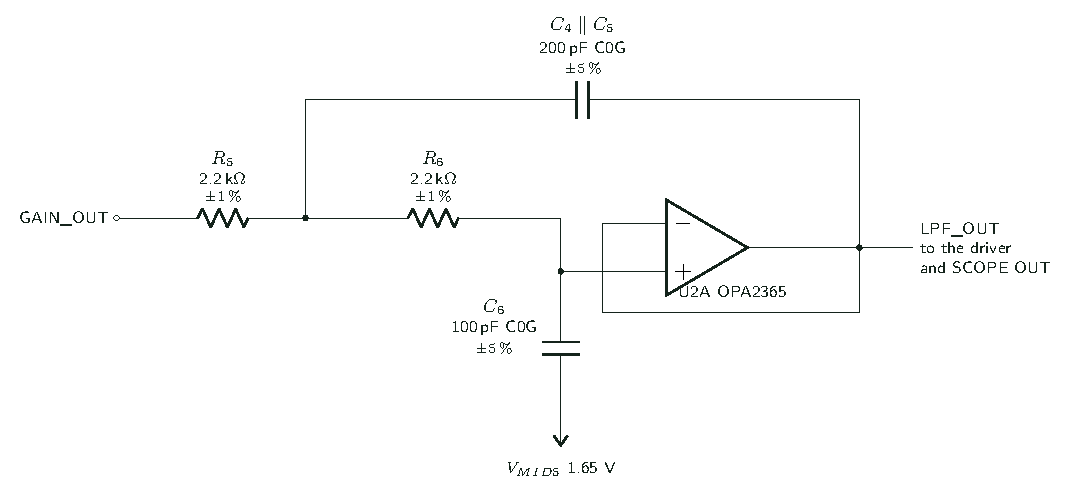
\includegraphics[width=0.98\textwidth]{s06_circuit.pdf}\end{center}
C4 and C5 (\SI{100}{pF} each) are in parallel, so they act as one $C_1=\SI{200}{pF}$. C6 is $C_2=\SI{100}{pF}$. U2A is a follower.

\section{Derivation from the node equations}
The output equals the $+$ input voltage: $V_o=V_B$ (deviations from VMID5).

\textbf{Node B}, no current into the $+$ input:
\[
\frac{V_B-V_A}{R_6}\cdot(-1)+V_B\,sC_6=0\;\Rightarrow\;V_A=V_B\,(1+sR_6C_6).
\]
\textbf{Node A:}
\[
\frac{V_A-V_{in}}{R_5}+\frac{V_A-V_B}{R_6}+sC_1\,(V_A-V_o)=0,\qquad V_o=V_B .
\]
Since $V_A-V_B=V_B\,sR_6C_6$, we have $(V_A-V_B)/R_6=V_B\,sC_6$ and $sC_1(V_A-V_B)=V_B\,s^2R_6C_1C_6$. Then
\[
V_A-V_{in}=-R_5V_B\,(sC_6+s^2R_6C_1C_6)
\;\Rightarrow\;
V_{in}=V_B\big[1+sC_6(R_5+R_6)+s^2R_5R_6C_1C_6\big].
\]
\[
\boxed{H(s)=\frac{1}{1+s\,C_6\,(R_5+R_6)+s^2\,R_5R_6C_1C_6}}
\qquad
\omega_0=\frac{1}{\sqrt{R_5R_6C_1C_6}},\quad
Q=\frac{\sqrt{R_5R_6C_1C_6}}{C_6\,(R_5+R_6)} .
\]
With $R_5=R_6=\SI{2.2}{k\ohm}$, $C_1=\SI{200}{pF}$, $C_6=\SI{100}{pF}$:
\[
f_0=\frac{1}{2\pi\cdot2.2\,\text{k}\Omega\sqrt{200\,\text{pF}\cdot100\,\text{pF}}}=\SI{511.5}{kHz},\qquad
Q=\frac{2.2\text{k}\sqrt{2\times10^{-20}}}{100\text{p}\cdot4.4\text{k}}=0.707 .
\]
It is the Butterworth low-pass: flat in the band, $-3$\,dB at $f_0$, and $-40$\,dB per decade above.

\begin{center}
\begin{tabular}{lrrrr}
\toprule
Frequency & \SI{250}{kHz} & \SI{500}{kHz} & \SI{800}{kHz} & \SI{2}{MHz}\\
\midrule
Loss of the low-pass alone & \SI{0.24}{dB} & \SI{2.8}{dB} & \SI{8.4}{dB} & \SI{23.8}{dB}\\
\bottomrule
\end{tabular}
\end{center}

\section{Aliasing: why a low-pass before the ADC}
A sampler at $F_S$ cannot tell $f$ from $|f-kF_S|$. The sample rate is about \SI{1.2}{MSPS} (estimate for a \SI{25}{MHz} SPI clock), so the fold frequency is $F_S/2=\SI{600}{kHz}$:
\[
f_\text{alias}=|f-F_S|:\quad \SI{700}{kHz}\to\SI{500}{kHz},\quad \SI{800}{kHz}\to\SI{400}{kHz},\quad \SI{1}{MHz}\to\SI{200}{kHz}.
\]
Noise above \SI{600}{kHz} would land inside the band if the filter did not remove it.

\begin{key}
Be honest about the margin: a second-order filter at \SI{512}{kHz} removes only \SI{8}{dB} at \SI{800}{kHz} and \SI{12}{dB} at \SI{1}{MHz}. The design relies on two facts. First, the measured event spectra fall steeply above \SI{300}{kHz}. Part of that fall came from the perfboard amplifier's own roll-off (its corner was \SI{0.31}{MHz}), so the real sensor spectrum may extend higher and needs a new measurement. Second, the corner is kept near the top of the band so the pass-band stays flat. A faster SPI clock (up to \SI{2.5}{MSPS}) moves the fold to \SI{1.25}{MHz} and adds margin.
\end{key}

\section{The whole filter chain}
The high-pass (slide 4) and the low-pass multiply, so in dB they add. The result is a band-pass with its $-3$\,dB points at \SI{106}{kHz} and \SI{502}{kHz} (ngspice, SENSOR IN to ADC). Total gain at \SI{250}{kHz} is \SI{12.3}{dB} ($\times4.1$): the gain stage's $4.9$, less the filter and driver losses. Loss at \SI{10}{kHz} is \SI{40.5}{dB} and at \SI{2}{MHz} \SI{24}{dB}.

\begin{center}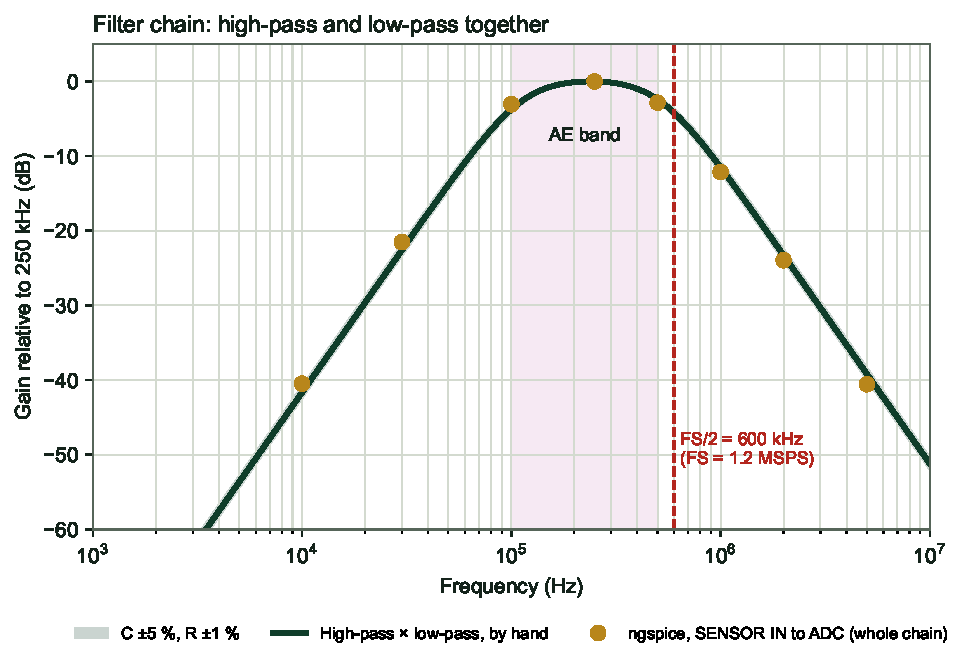
\includegraphics[width=0.82\textwidth]{s06_graph.pdf}\end{center}
The hand model (high-pass times low-pass) and the full ngspice chain agree within \SI{1.1}{dB} at every point shown.

\section{Tolerances}
C0G capacitors $\pm5\,\%$ (C14858), resistors $\pm1\,\%$ (C4190). Over all 16 corners:
\[
f_0=\SI{482}{} \text{ to } \SI{544}{kHz},\qquad Q=0.673\text{ to }0.743 .
\]
The upper corner moves about $\pm6\,\%$ and stays above the band edge. $Q$ changes the shape slightly, with at most about \SI{0.4}{dB} of droop near the corner.
\end{document}
